%% AI INTERPRETATION: This document appears to be a scientific presentation on computing digits of π via collisions in an idealized billiard system. Slide markers denote individual frames; headings and lists within each slide define titles and content. Images are placed as scalable placeholders with comments for replacements.

\documentclass{beamer}
\usepackage[utf8]{inputenc}
\usepackage[brazil]{babel}
\usepackage{graphicx}
\usepackage{amsmath,amssymb}
\usetheme{metropolis} % modern, clean theme

% Document metadata inferred from Slide 1
\title{Jogando Sinuca com $\pi$}
\subtitle{Como o número de colisões em um sistema mecânico computa os dígitos de $\pi$}
\author{Leonardo Lima Santos \\ Lucas Pimentel Alves da Costa \\ Pedro Kury Kitagawa}
\date{\today}

\begin{document}

\maketitle

% Slide 2
\begin{frame}{Definição do Problema}
  \textbf{Objetivo:} Calcular a quantidade de colisões em um sistema idealizado
  \begin{itemize}
    \item \textbf{Sistema Físico}
      \begin{itemize}
        \item Parede fixa em $x = 0$
        \item Duas bolas de massa $m$ (pequena) e $M$ (grande)
        \item Movimento unidimensional (eixo $X$)
        \item Bola $m$ em repouso entre parede e bola $M$
        \item Bola $M$ inicia com velocidade $V$ em direção a $m$
      \end{itemize}
  \end{itemize}
\end{frame}

% Slide 2+1
\begin{frame}{Definição do Problema}
  \begin{figure}
    \centering
    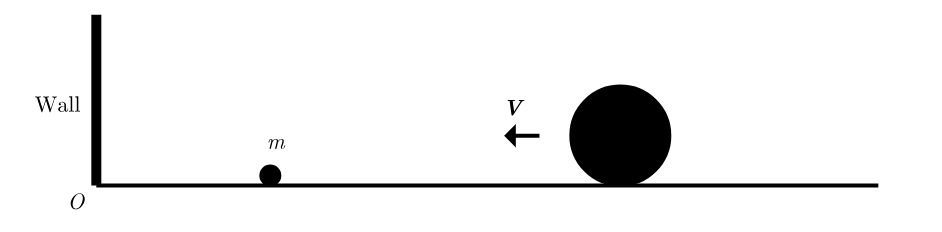
\includegraphics[width=1\textwidth]{images/image.png}
  \end{figure}
\end{frame}

% Slide 3
\begin{frame}{Variáveis e Suposições do Sistema}
  \begin{itemize}
    \item Variáveis fundamentais:
      \begin{itemize}
        \item Massa das bolas $m$ e $M$
        \item Razão $\tfrac{M}{m} = 100^N$, com $N$ dígitos de $\pi$ a computar
      \end{itemize}
    \item Simplificações e desconsiderações:
      \begin{itemize}
        \item Colisões perfeitamente elásticas
        \item Ausência de atrito e resistência do ar
        \item Bolas como partículas adimensionais
      \end{itemize}
  \end{itemize}
\end{frame}

% Slide 4
\begin{frame}{O que realmente acontece nas colisões?}
  \textbf{Análise do caso simples $m = M$}
  \begin{equation*}
    \begin{alignedat}{2}
      u_0 &= 0,                           &\qquad v_0 &= V, \\
      u_1 &= \frac{(m - M)u_0 + 2Mv_0}{m + M}, & v_1 &= \frac{(M - m)v_0 + 2mu_0}{m + M}
    \end{alignedat}
  \end{equation*}
\end{frame}

% Slide 5
\begin{frame}{Resultados para $m = M$}
  \begin{equation*}
    \begin{aligned}
      u_1 &= \frac{2MV}{2M} = V, \\
      v_1 &= \frac{0 \cdot V}{2m} = 0
    \end{aligned}
  \end{equation*}
  \begin{enumerate}
    \item $M$ bate com velocidade $V$ na bola $m$ e fica em repouso (1ª colisão)
    \item $m$ segue até a parede, bate na parede com velocidade $V$ e volta com velocidade $-V$ (2ª colisão)
    \item $m$ bate com velocidade $-V$ na bola $M$ e fica em repouso (3ª colisão)
    \item $M$ segue com $-V$ indefinidamente
  \end{enumerate}
\end{frame}

% Slide 6
\begin{frame}{O espaço de configuração do sistema}
  Posição da \textbf{bola} $\mathbf{m}$ é $\mathbf{x=x(t)}$, e da \textbf{bola} $\mathbf{M}$ é $\mathbf{y=y(t)}$
  
  Definimos como \textbf{função posição} $P(t) = (x(t), y(t))$, com $0 \le x(t) \le y(t)$, que nos dá um ponto em um espaço no $\mathbb{R}^2$

  \begin{figure}
    \centering
    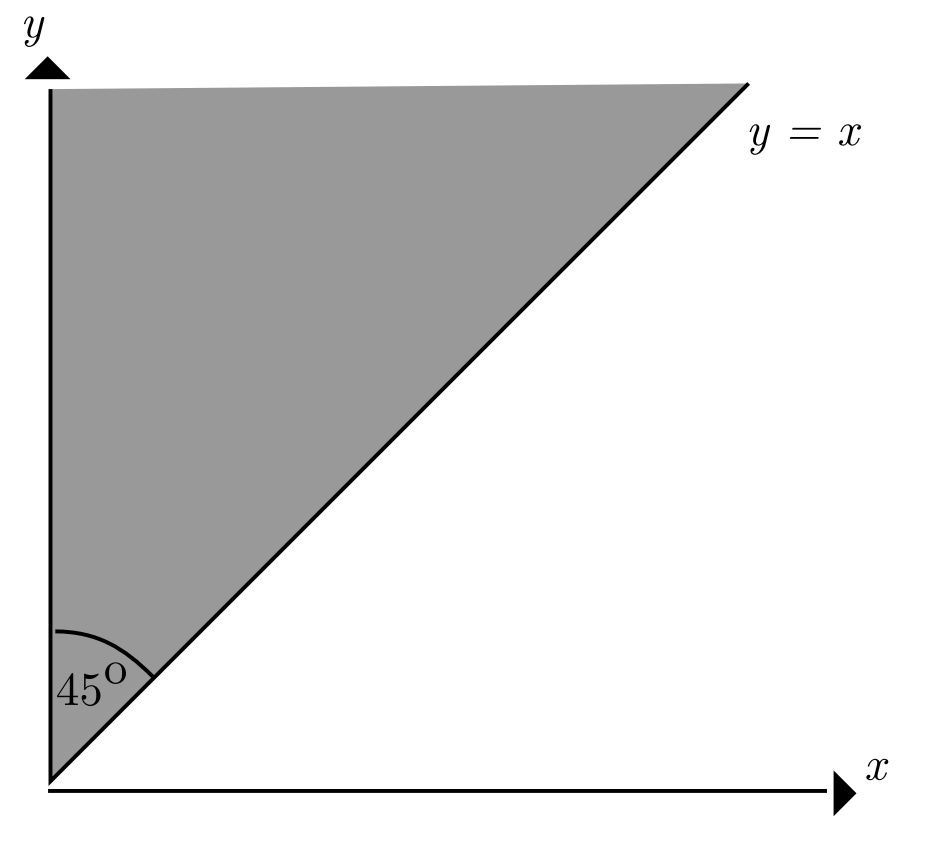
\includegraphics[width=0.6\textwidth]{images/image1-1.png}
  \end{figure}
\end{frame}

% Slide 7
\begin{frame}{Tipos de Colisões no Sistema}
  \begin{itemize}
    \item \textbf{Bola-Parede}: $x(t)=0$, reflexão simples no eixo $Y$
    \item \textbf{Bola-Bola}: $x(t)=y(t)$, reflexão na fronteira $x=y$ (a depender das massas)
  \end{itemize}
  No caso em que $m=M$, as reflexões são todas ópticas.
\end{frame}

% Slide 8
\begin{frame}{Início do experimento}
  $\vec{P}=(x(t), y(t))$, $\dot{\vec{P}}=(\dot x,\dot y)=(u, v)$
  \begin{figure}
    \centering
    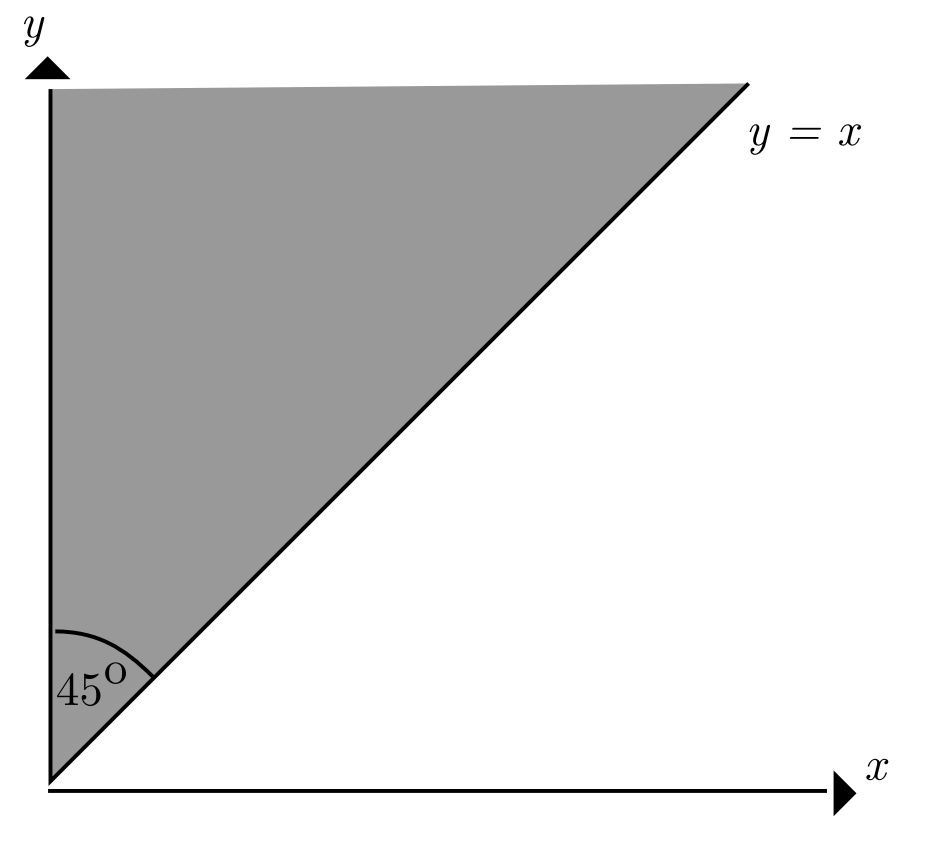
\includegraphics[width=0.7\textwidth]{images/image1-1.png}
  \end{figure}
\end{frame}

% Slide 9
\begin{frame}{Primeira colisão entre $m$ e $M$}
  $\dot{\vec{P}}(t_0)=(0,V)\to\dot{\vec{P}}(t_1)=(V,0)$
  \begin{figure}
    \centering
    % Placeholder: replace with images/image1-2.png
    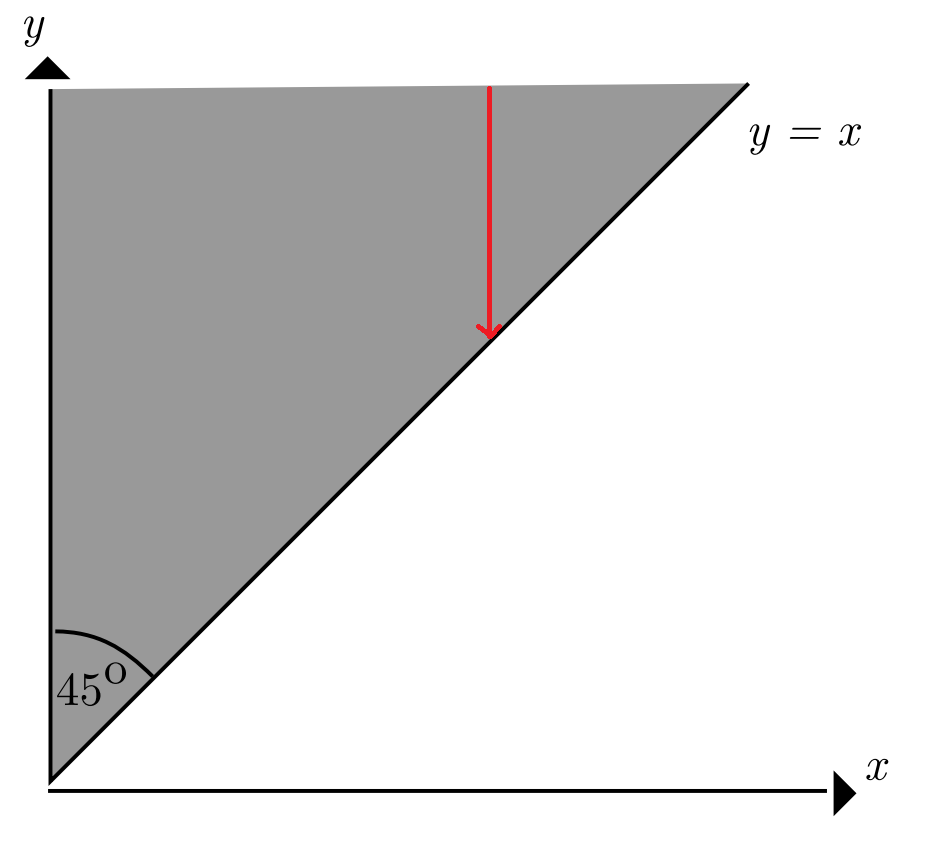
\includegraphics[width=0.7\textwidth]{images/image1-2.png}
  \end{figure}
\end{frame}

% Slide 10
\begin{frame}{Colisão entre $m$ e a parede}
  $\dot{\vec{P}}(t_1)=(V,0)\to\dot{\vec{P}}(t_2)=(-V,0)$
  \begin{figure}
    \centering
    % Placeholder: replace with images/image1-3.png
    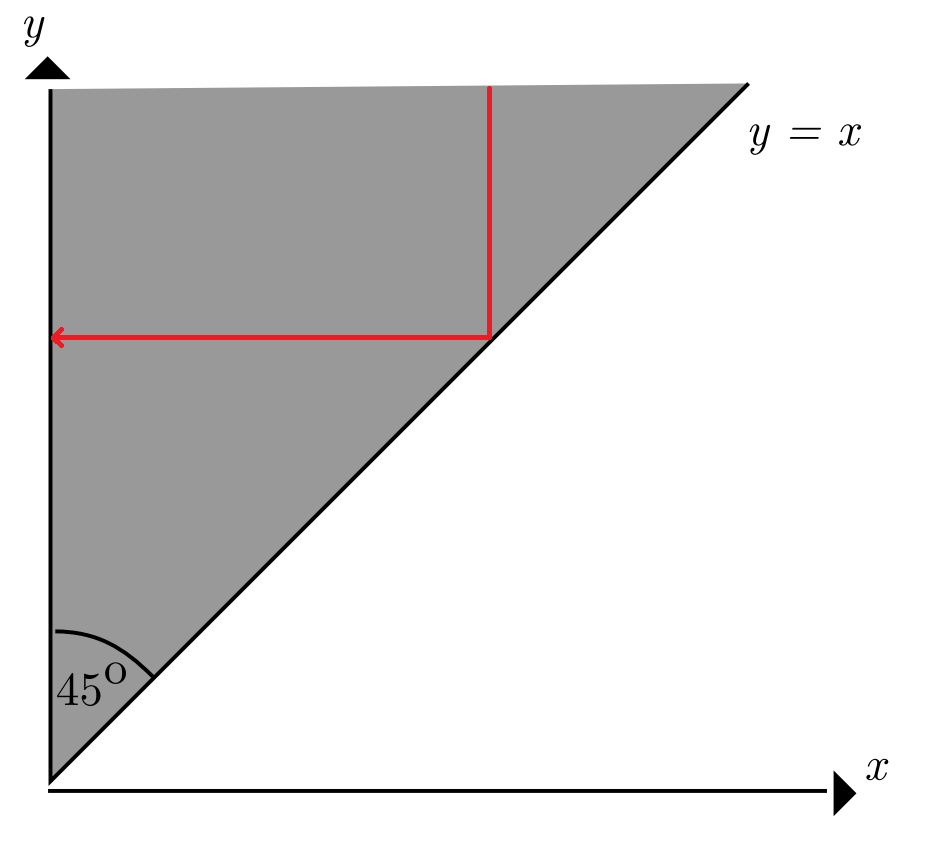
\includegraphics[width=0.8\textwidth]{images/image1-3.png}
  \end{figure}
\end{frame}

% Slide 11
\begin{frame}{Segunda colisão entre $m$ e $M$}
  $\dot{\vec{P}}(t_2)=(-V,0)\to\dot{\vec{P}}(t_3)=(0,-V)$
  \begin{figure}
    \centering
    % Placeholder: replace with images/image1-4.png
    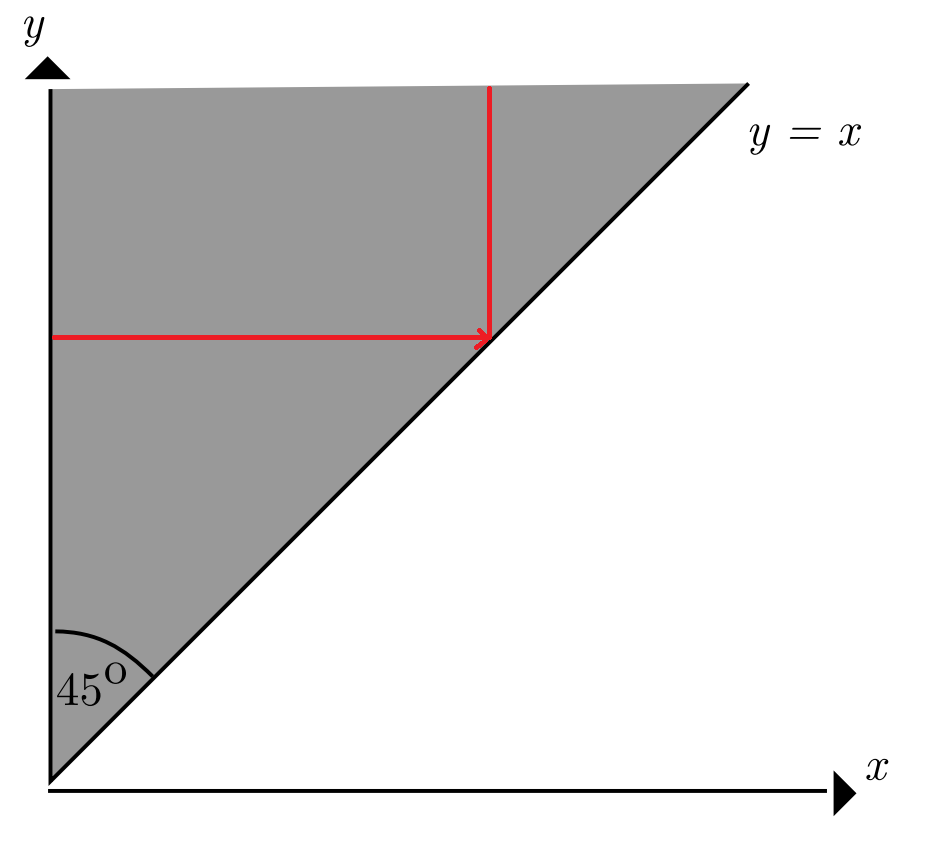
\includegraphics[width=0.7\textwidth]{images/image1-4.png}
  \end{figure}
\end{frame}

% Slide 12
\begin{frame}{$M$ segue infinitamente, com $m$ parado}
  $\dot{\vec{P}}(t_{\infty})=(0,-V)$
  \begin{figure}
    \centering
    % Placeholder: replace with images/image1-5.png
    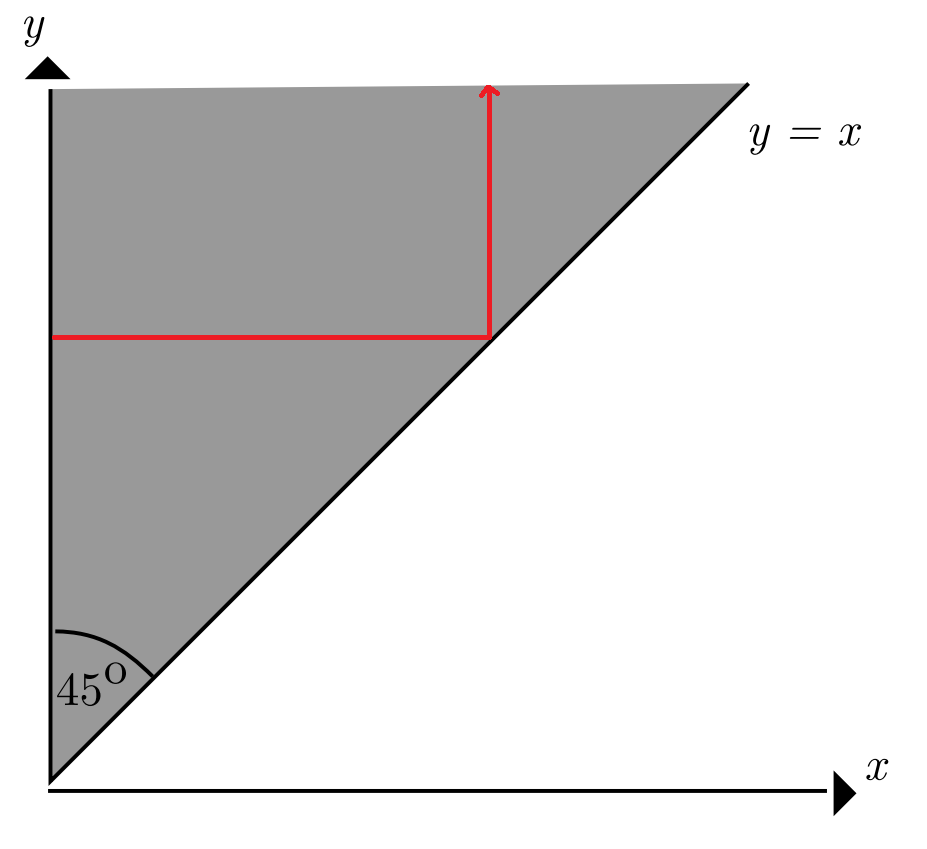
\includegraphics[width=0.6\textwidth]{images/image1-5.png}
  \end{figure}
\end{frame}

% Slide 13
\begin{frame}{O que acontece quando $m \neq M$?}
  \begin{itemize}
    \item Reflexões não são ópticas
    \item Não sabemos se as colisões param
  \end{itemize}
  \begin{figure}
    \centering
    % Placeholder: replace with images/image-2.png
    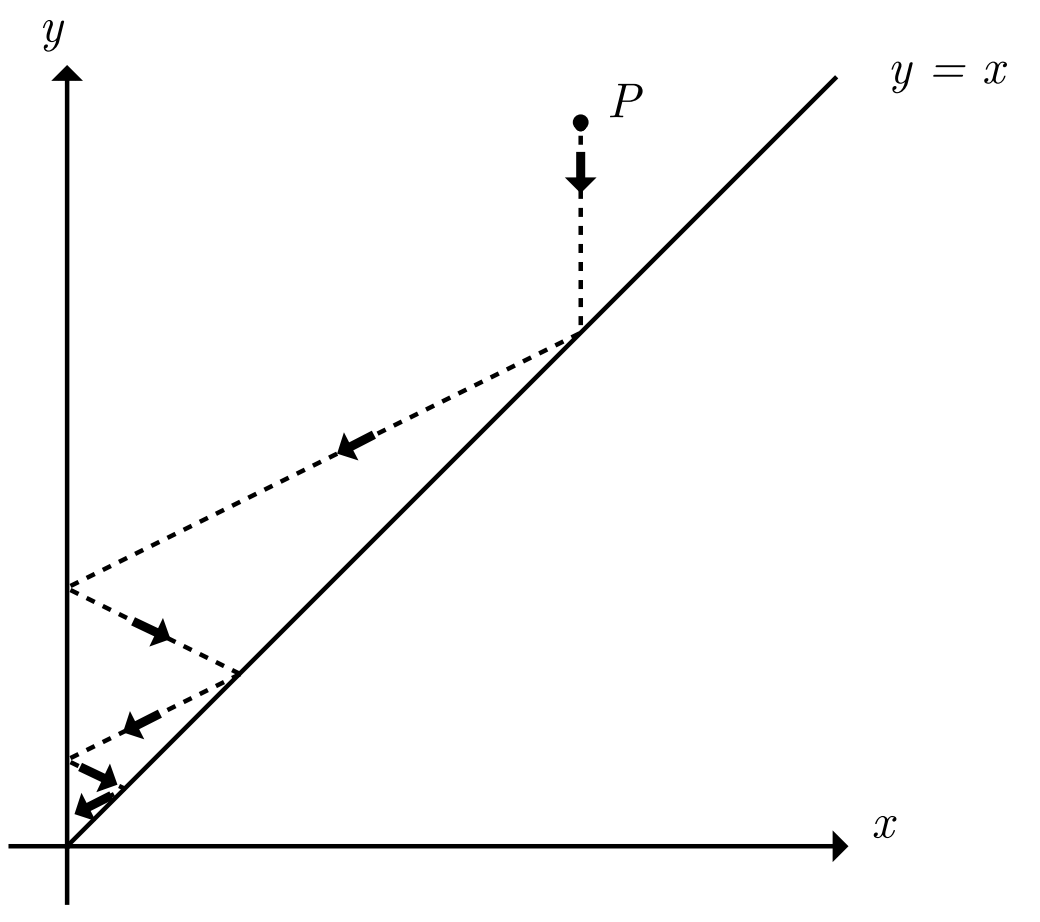
\includegraphics[width=0.65\textwidth]{images/image-2.png}
  \end{figure}
\end{frame}

% Slide 14
\begin{frame}{O pulo do gato}
  \textbf{A chave para simplificar o problema}: tornar a reflexão na fronteira $x=y$ óptica (i.e., o ângulo de entrada igual ao de saída). Definimos:
  \begin{equation*}
    x' = \sqrt{m}\,x,\quad y' = \sqrt{M}\,y
  \end{equation*}
\end{frame}

% Slide 15
\begin{frame}{Representação Matricial da Transformação}
  \begin{gather*}
    %--- Primeiro grupo de alinhamento ---
    \begin{alignedat}{2}
      \vec{P} &= \begin{pmatrix} x \\ y \end{pmatrix}, &\qquad \vec{P'} &= \begin{pmatrix} x' \\ y' \end{pmatrix}
    \end{alignedat}
    \\[2ex] % Espaçamento vertical entre os grupos
    %--- Segundo grupo de alinhamento ---
    \begin{alignedat}{2}
      T &= \begin{pmatrix} \sqrt{m} & 0 \\ 0 & \sqrt{M} \end{pmatrix}, &\qquad \vec{P'} &= T\,\vec{P}
    \end{alignedat}
  \end{gather*}

  Resultando em:
  \begin{equation*}
    \vec{P'}=\begin{pmatrix}\sqrt m\,x\\\sqrt M\,y\end{pmatrix}
  \end{equation*}
\end{frame}

% Slide 17
\begin{frame}{Novo espaço após aplicação de $T$}
  Ângulo entre eixo $X$ e reta $x=y$ se altera.
  \begin{figure}
    \centering
    % Placeholder: replace with images/image-3.png
    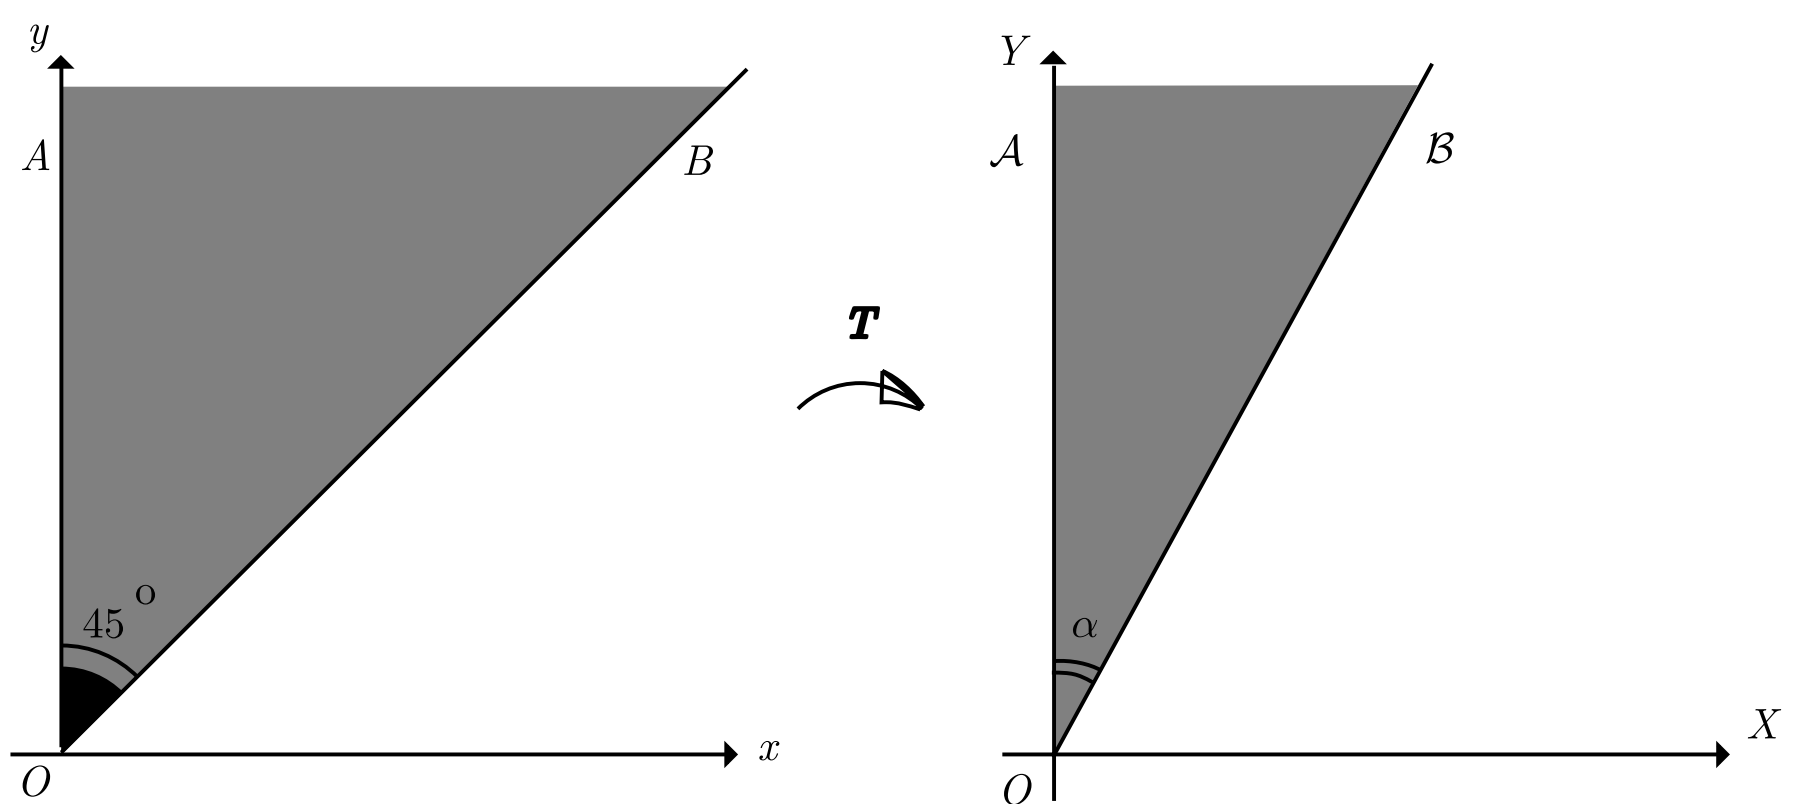
\includegraphics[width=1\textwidth]{images/image-3.png}
  \end{figure}
\end{frame}

% Slide 18
\begin{frame}{Por que aplicamos $T$?}
  \begin{itemize}
    \item \textbf{Objetivo:} fazer com que as reflexões tornem-se ópticas
    \item Precisamos, então, provar que $T$ faz com que as reflexões sejam ópticas
  \end{itemize}
\end{frame}

% Slide 19
\begin{frame}{Propriedades da Transformação $T$}
  \textbf{Velocidade:} ${\dot{\vec{P'}}}=(\sqrt{m}u,\sqrt{M}v)$. Em outras palavras, $T$ transforma a velocidade da mesma
  forma que transforma as posições.
  Vamos analisar as reflexões nos seguintes casos:
  \begin{itemize}
    \item Reflexão na parede (fixada em $x=0$)
    \item Reflexão no eixo $Y=\sqrt{\frac{M}{m}}\,X$
  \end{itemize}
\end{frame}


% Slide 20
\begin{frame}{Ângulo Transformado}
  Quando aplicamos $T$ no espaço, o nosso novo ângulo $\alpha$ é tal que: 
  $$\tan{\alpha}=\frac{x'}{y'}=\frac{\sqrt{m}\cdot x}{\sqrt{M}\cdot y}=\sqrt{\frac{m}{M}}$$
  
  já que $y=x$ no lado oblíquo ao ângulo. Logo $\alpha = \arctan{\sqrt{\frac{m}{M}}}$. Usaremos isso no futuro.
\end{frame}

% Slide 21
\begin{frame}{Reflexão no eixo $Y$}
  Vamos chamar de $\varphi$ o ângulo que a trajetória faz com o eixo $Y$ antes de atingí-lo e chamar de $\psi$ o ângulo que a trajetória faz com o eixo $Y$ depois de tê-lo atingido. 
  
  A mudança da velocidade $u$ para $-u$ implica na transformação 
  \begin{equation*}
    \dot{\vec{P'}}=(-\sqrt m\,u,\sqrt M\,v)
  \end{equation*}

  Isso só pode acontecer se $\varphi=\psi$.
\end{frame}

% Slide 22
\begin{frame}{Demonstração: Reflexão no Eixo Y}
  \begin{figure}
    \centering
    % Placeholder: replace with images/image-4.png
    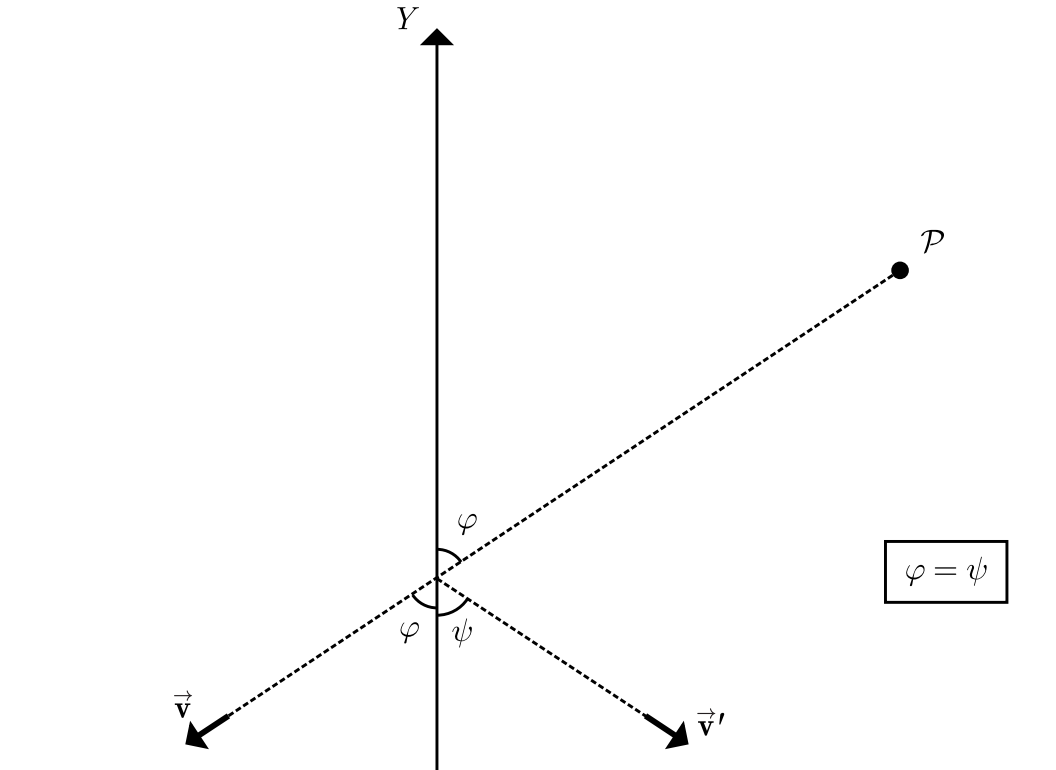
\includegraphics[width=0.8\textwidth]{images/image-4.png}
  \end{figure}
  Conclui-se que é reflexão óptica. $\square \, 1/2$ 
\end{frame}

% Slide 23
\begin{frame}{Reflexão no eixo $Y=\sqrt{\tfrac{M}{m}}X$}
  Considerando as conservações do sistema, entenda $K_1$ e $K_2$ como constantes tal que:
  \begin{equation*}
    \begin{cases}mu+Mv&=K_1,\text{(conservação do momento linear)} \\mu^2+Mv^2&=K_2,\text{(conservação da energia cinética)} \end{cases}
  \end{equation*}
\end{frame}

% Slide 24
\begin{frame}{Reformulações em Coordenadas Transformadas}
  $$
  \dot{\vec{P'}}=(\sqrt m\,u,\sqrt M\,v)
  $$
  $$
  \vec m=(\sqrt{m},\sqrt{M})
  $$
  \begin{equation*}
    \begin{cases}\vec m\cdot\dot{\vec{P'}}=K_1,\\|\dot{\vec{P'}}|^2=K_2.\end{cases}
  \end{equation*}

  Dessa forma:
  $$|\vec{m}| |\dot{\vec{P'}}| \cos{\varphi} = K_1 \therefore$$
  $$(\sqrt{M+m}) \sqrt{K_2} \cos{\varphi} = K_1$$
\end{frame}

% Slide 25
\begin{frame}{Demonstração: Reflexão na Diagonal}
  Então:
  $\cos{\varphi} = \frac{K_1}{(\sqrt{M+m}) \sqrt{K_2}} = K_3$, com $K_3$ constante.
  \begin{itemize}
    \item Depois da reflexão, o ângulo passa a ser $\psi$, mas o mesmo sistema ainda vale, então $\cos{\psi} = K_3$
    \item Concluímos, portanto, que $\psi = \varphi$
  \end{itemize}
  $\blacksquare \, 2/2$
\end{frame}

% Slide 26
\begin{frame}{Número de Reflexões Ópticas}
  Até agora, o número de reflexões ainda pode ser infinita. 
  Enunciamos, e em seguida provaremos, o seguinte lema:
  \begin{block}{Lema}
    (a) Máximo número de reflexões no ângulo $\alpha$ é finito.\\
    (b) O número de reflexões é igual a $\frac{\pi}{\alpha}$ se $\frac{\pi}{\alpha}\in\mathbb Z$, senão $\lfloor\frac{\pi}{\alpha}\rfloor+1$.\\
    (c) Se o raio inicial for paralelo a um dos lados do ângulo $\alpha$ (ou seja, $u=0,v=V$), o número reduz em 1.
  \end{block}
\end{frame}

% Slide 27
\begin{frame}{Desdobramento}
  Desdobramos o ângulo $\alpha$ e a trajetória $\gamma$. Como as reflexões são ópticas, então a imagem é a reta $k$.
  \begin{figure}
    \centering
    % Placeholder: replace with images/image-5.png
    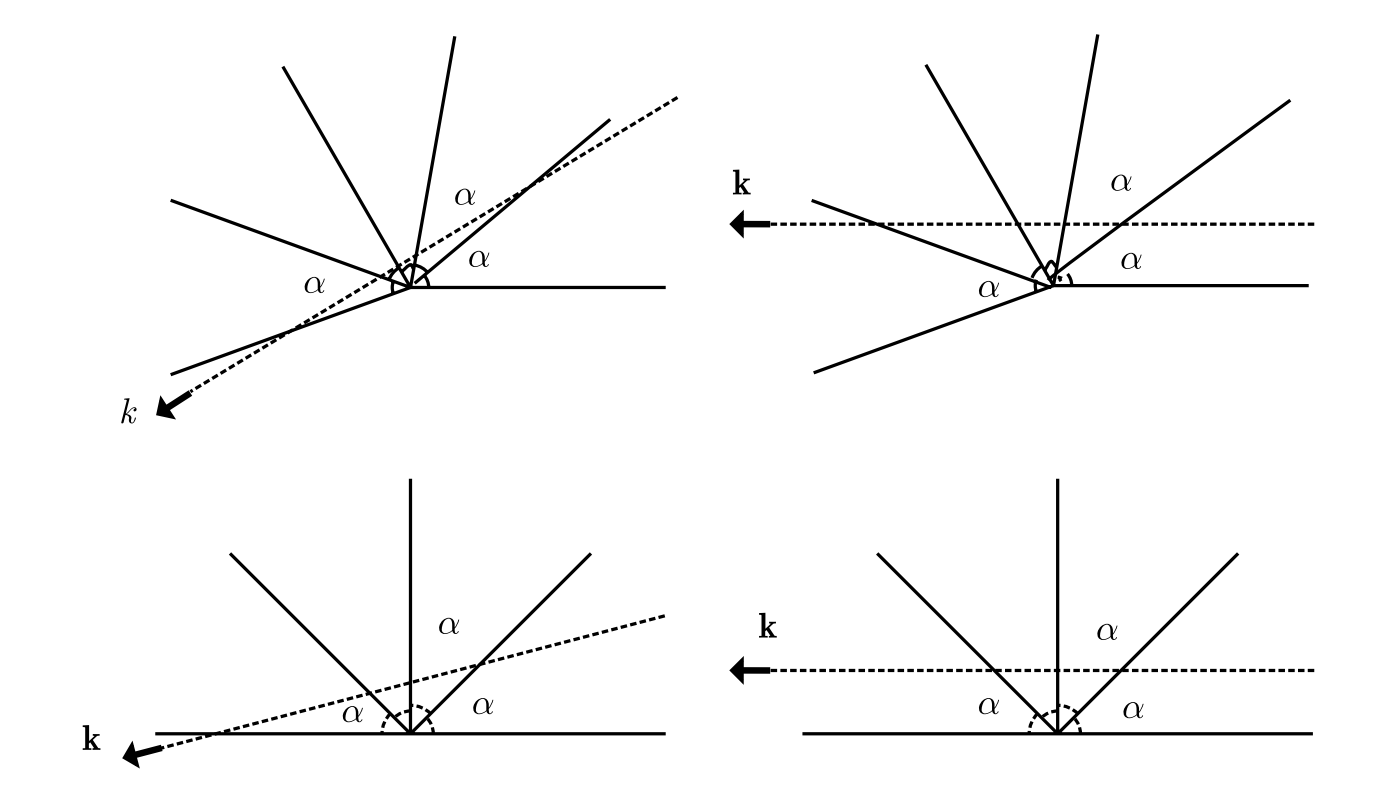
\includegraphics[width=1\textwidth]{images/image-5.png}
  \end{figure}
\end{frame}

% Slide 28
\begin{frame}{Prova do Lema}
  Para cada intersecção de $k$ com uma cópia do ângulo, acontece uma reflexão em $\gamma$.
  
  \begin{itemize}
    \item Como $k$ intersecta uma quantidade finita de ângulos, então está provado (a). $\square \, 1/3$
    \item Se $n$ é o número máximo de reflexões, temos $n\alpha=\pi$, ou $n\alpha >\pi>(n-1)\alpha$. No primeiro caso, $n = \frac{\pi}{\alpha}$, no segundo caso, $n = [\frac{\pi}{\alpha}]+1$. $\square \, 2/3$
    \item Quando $k$ é paralelo ao lado do ângulo $\alpha$, então a possível intersecção final não acontece. $\blacksquare \, 3/3$
  \end{itemize}

\end{frame}

% Slide 29
\begin{frame}{Prova do Teorema $\Pi=31415926535897\dots$}
    \begin{itemize}
      \item Tome o número de reflexões $\Pi(N)$.
      \item Suponha o raio $k$ que descreve o desdobramento da trajetória $\gamma$ do sistema na configuração $\alpha = AOB$.
    \end{itemize}
\end{frame}

% Slide 29 + 1
\begin{frame}{Prova do Teorema $\Pi=31415926535897\dots$}
  \begin{column}{0.4\textwidth}
    O início de $\gamma$ (i.e., antes do primeiro choque) deve ser paralelo ao eixo $Y$ (ou seja, $u = 0$ e $v = V$), assim como $k$.
  \end{column}
  \begin{column}{0.6\textwidth}
      \begin{figure}
        \centering
        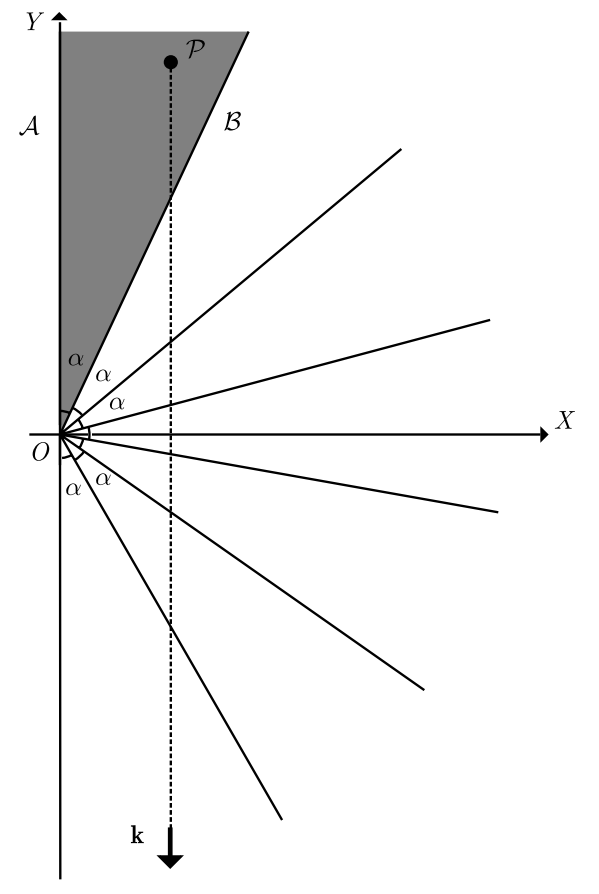
\includegraphics[width=0.8\textwidth]{images/image5.png}
      \end{figure}
  \end{column}
\end{frame}

% Slide 29 + 2
\begin{frame}{Prova do Teorema $\Pi=31415926535897\dots$}
  Dessa maneira, o número de reflexões nos "lados do ângulo $\alpha$" é igual a $\lfloor\pi/\alpha\rfloor$, mas nada garante que $\pi/\alpha$ será um número inteiro, na verdade:

    $$
    \alpha = \arctan{\sqrt{\frac{m}{M}}} = \arctan{\sqrt{\frac{m}{m \cdot 100^N}}} = \arctan{(10^{-N})}
    $$
\end{frame}

% Slide 31
\begin{frame}{Fórmula para $\Pi$: O caso simples}
    Para $N=0$:
    $$
    \alpha  = \arctan(10^0) = \arctan(1) = \frac{\pi}{4}
    $$
    \vspace{}
    Então a primeira parte do Lema (c) vale: 
    $$
    \Pi(0)=\lfloor4\rfloor - 1 = 3
    $$
\end{frame}

% Slide 32
\begin{frame}{Fórmula para $\Pi$: Demais Casos}
    Para $N\ge1$, $\alpha = \arctan(10^{-N})$ é um ângulo arbitrário que não consegue mensurar um número racional de graus $(180/k)\degree$. Nesse contexto, a segunda parte do Lema (c) é aplicável e consequentemente achamos a fórmula exata:
    
    $$
    \Pi(N) = \left\lfloor\frac{\pi}{\arctan(10^{-N})}\right\rfloor_{\,\,\,\blacksquare}
    $$
    
    Podemos realizar uma aproximação para $\arctan(10^{-N})$ para simplificar a nossa solução exata. 
\end{frame}

% Slide 33
\begin{frame}{Aproximação usando Série de Taylor}
    Recorde-se que:
    
    $$
    \arctan{x} = \int^x_0{\frac{dt}{1+t^2}} = \int^x_0 \sum^{\infty}_{n=0}(-t^2)^ndt = \sum^{\infty}_{n=0}\frac{(-1)^nx^{2n+1}}{2n+1}
    $$
    
    $$
    \arctan{x} = x - \frac{x^3}{3} + \frac{x^5}{5} - \frac{x^7}{7} + \dots
    $$
\end{frame}

% Slide 34
\begin{frame}{Limite da Aproximação}
  Usando a aproximação anterior, podemos afirmar que:
$$
\lim_{x\rightarrow 0}\left( \frac{1}{\arctan{x}} - \frac{1}{x} \right)= 0
$$

Então, $\arctan(x) \approx x$ quando $x \rightarrow 0$
\end{frame}

% Slide 35
\begin{frame}{Aproximação para $\Pi$: Demais Casos (continuação)}
Como $x = 10^{-N}$ e $N \in \mathbb{N}$, temos que:
$$
1\geq x>0
$$
e:
$$
\frac{1}{\arctan{x}} > \frac{1}{x} \implies \frac{\pi}{\arctan{x}} > \frac{\pi}{x}
$$


Como $\frac{\pi}{\arctan(10^{-N})}>\frac{\pi}{10^{-N}}$, logo:

$$
\Pi(N) = \left\lfloor \frac{\pi}{\arctan(10^{-N})}\right\rfloor\approx \left\lfloor \frac{\pi}{10^{-N}}\right\rfloor = \lfloor\pi \cdot 10^{N}
\rfloor$$

\end{frame}

% Slide 36
\begin{frame}{Precisão da Aproximação}
  Empiricamente, pode-se verificar que $\Pi(N) = \left\lfloor\pi*10^N\right\rfloor$ para $N \le 50,000,000$. Contudo, para $N > 50,000,000$ algo particular do método deve ser considerado.
\end{frame}

% Slide 37
\begin{frame}{Problema no método}
    Da demonstração anterior, temos que:
  $$
  \lim_{N\to\infty}\left(\frac{\pi}{\arctan(10^{-N})}-\frac{\pi}{10^{-N}}\right)=0
  $$
  Portanto, pelo Lema (b) e pelo Lema (c), temos duas opções para quando $N$ é grande.
\end{frame}

% Slide 38
\begin{frame}{Análise das Duas Opções de Erro}
  \begin{itemize}
    \item Opção 1 (Lema c): 
    $$\Pi(N) = \left [ \frac{\pi}{\arctan{(10^{-N})}}\right] = [\pi 10^N]$$
    $$\Pi(N) = [(3.1415\dots a_{N-1} a_{N})10^N]=31415\dots a_{N-1}a_N$$
    \item Opção 2 (Lema b): 
    $$\Pi(N) = \left [ \frac{\pi}{\arctan{(10^{-N})}}\right] = [\pi 10^N]+1$$
    $$\Pi(N) =[(3.1415\dots a_{N-1} a_{N})10^N]=31415\dots a_{N-1}a_N+1$$
  \end{itemize}
\end{frame}

% Slide 39
\begin{frame}{Continuação da Análise de Erro}
  Então, o nosso erro pode ser descrito da seguinte maneira:
    \begin{equation*}
        \Pi(N) - \lfloor \pi \cdot 10^N \rfloor = \left\{
        \begin{array}{c}
        0 \\
        1
        \end{array}
        \right.
    \end{equation*}

Entretanto, o número de dígitos errados pode ser maior caso existam $k$ dígitos 9 seguidos ao final do número.
\end{frame}
% Slide 40
\begin{frame}[allowframebreaks]{Referências}
  \begin{thebibliography}{}
    \bibitem{Galperin2003} G. Galperin, \emph{Playing Pool with π}, 9 dez. 2003.
    \bibitem{3blue1brown2019} 3Blue1Brown, \emph{The most unexpected answer to a counting puzzle}, YouTube, 13 jan. 2019.
    \bibitem{3blue1brown2025} 3Blue1Brown, \emph{There's more to those colliding blocks that compute pi}, YouTube, 13 mar. 2025.
    \bibitem{StandUpMaths2025} Stand-Up Maths, \emph{We calculated pi with colliding blocks}, YouTube, 13 mar. 2025.
  \end{thebibliography}
\end{frame}

\end{document}